\section{Phân tích và Đánh giá Kết quả Thực nghiệm}
\label{sec:4_2_results}

Mục này trình bày kết quả thực nghiệm chi tiết đánh giá thuật toán Mạng Khí Nơ-ron Tăng trưởng Tích lũy Bằng chứng (Evidence-Accumulating Growing Neural Gas - EAGNG) trong bài toán phân loại lỗi tự động trên màn hình điện thoại. Việc đánh giá được thực hiện thông qua bốn nội dung chính bao gồm: (i) khả năng thích ứng với dịch chuyển khái niệm (Concept Drift), (ii) độ ổn định cấu trúc và hiện tượng quên thảm họa, (iii) thời gian xử lý và tốc độ thực thi, và (iv) hiệu quả phân cụm không gian hình học của không gian biểu diễn lỗi.

\subsection{Đánh giá khả năng thích ứng với dịch chuyển khái niệm}
\label{sec:4_2_1_concept_drift}

Khả năng thích ứng với dữ liệu chuỗi theo thời gian đóng vai trò quyết định đối với các mô hình học trực tuyến trong môi trường sản xuất công nghiệp. Thực nghiệm mô phỏng chuỗi dữ liệu gồm $3000$ mẫu với bốn điểm dịch chuyển khái niệm tại các thời điểm mẫu thứ $600$, $1200$, $1800$, và $2400$, tương ứng với sự xuất hiện của các dạng lỗi mới như đường kẻ ngang, hình tam giác, đường kẻ dọc, và hình chữ nhật. Kết quả đánh giá chỉ số điều chỉnh Rand (Adjusted Rand Index - ARI) thể hiện sự vượt trội của phương pháp đề xuất so với các thuật toán cơ sở.

\begin{figure}[htbp]
    \centering
    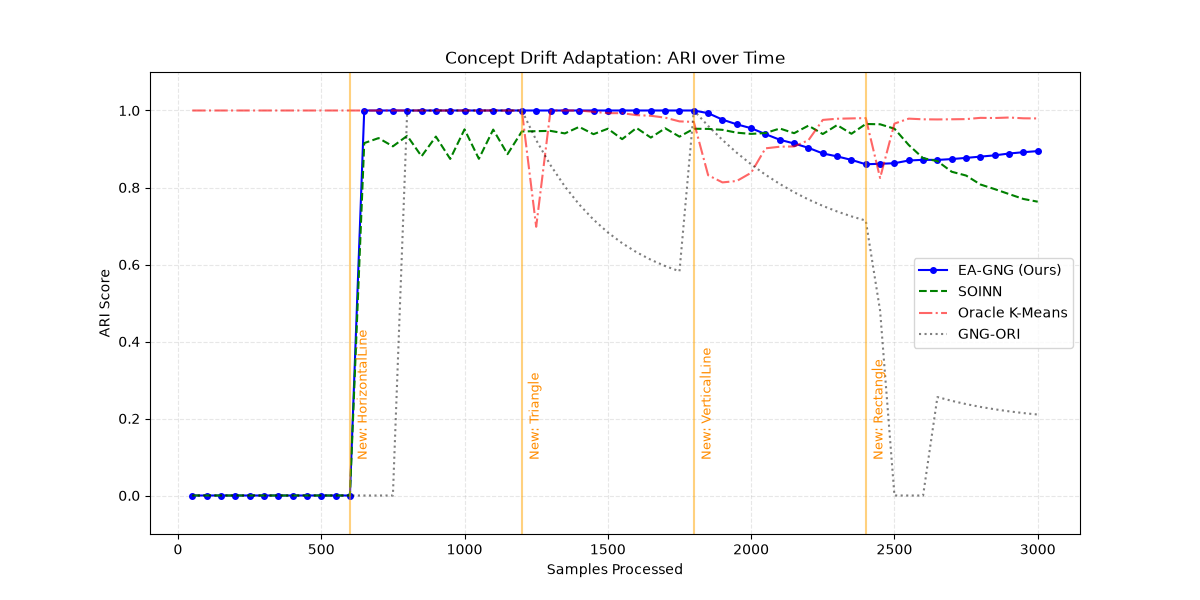
\includegraphics[width=0.9\linewidth]{figures/c4/c4_ARI.png}
    \caption{Sự biến thiên của chỉ số điều chỉnh Rand theo thời gian khi xuất hiện các dạng lỗi mới.}
    \caption*{Ghi chú: Đường nét liền màu xanh thể hiện phương pháp EAGNG, đường nét đứt màu xanh lá thể hiện SOINN, đường chấm chấm màu xám thể hiện GNG truyền thống, và đường gạch chấm màu đỏ thể hiện Oracle K-Means.}
    \label{fig:drift_ari}
\end{figure}

Như thể hiện trong Hình~\ref{fig:drift_ari}, chỉ số điều chỉnh Rand của thuật toán EAGNG nhanh chóng hội tụ về giá trị xấp xỉ $100\%$ ngay sau khi xuất hiện các dạng lỗi mới tại thời điểm $600$, $1200$, và $1800$. Đối với phương pháp GNG truyền thống \cite{fritzke1995growing}, chỉ số Rand suy giảm nghiêm trọng sau thời điểm $2400$, rơi xuống mức $21{,}0\%$ tại thời điểm $3000$ do hiện tượng nhiễu cấu trúc và không thể tách biệt các cụm lỗi trùng lặp. Phương pháp SOINN \cite{furao2006soinn} duy trì được tính ổn định tương đối nhưng chỉ đạt chỉ số Rand bằng $76{,}3\%$ tại bước $3000$, do cơ chế thiết lập ngưỡng bán kính cố định dẫn đến việc chia nhỏ các cụm lỗi tự nhiên.

\begin{figure}[htbp]
    \centering
    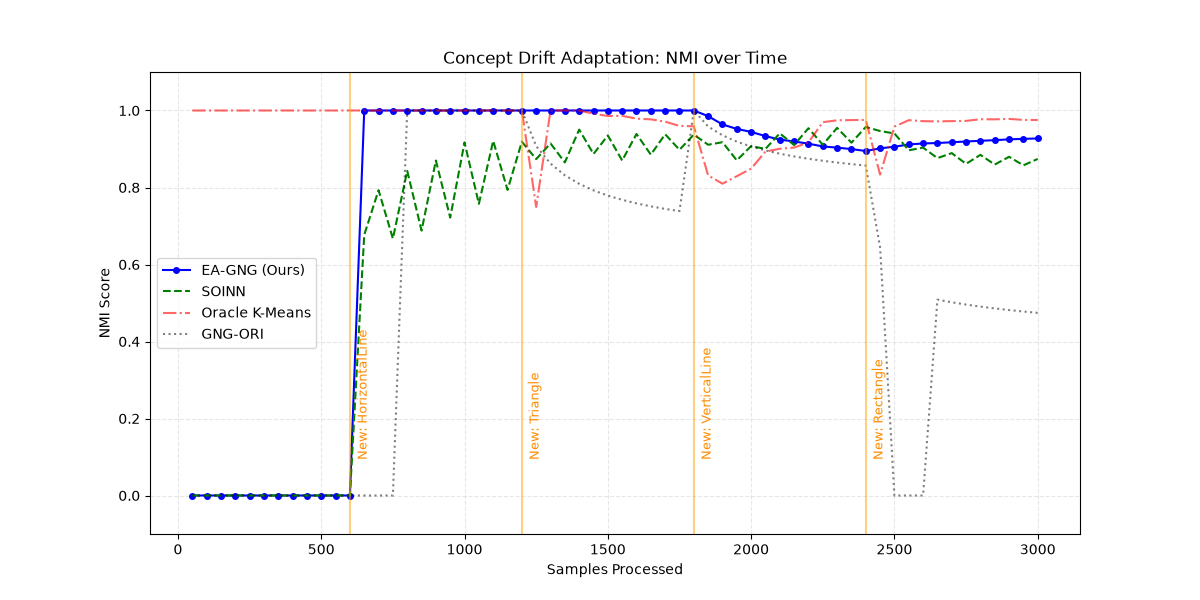
\includegraphics[width=0.9\linewidth]{figures/c4/c4_NMI.png}
    \caption{Sự biến thiên của chỉ số thông tin tương hỗ chuẩn hóa theo chuỗi thời gian xử lý mẫu.}
    \caption*{Ghi chú: Đánh giá khả năng bảo toàn thông tin phân cụm giữa kết quả của mô hình và nhãn thực tế.}
    \label{fig:drift_nmi}
\end{figure}

Chỉ số thông tin tương hỗ chuẩn hóa (Normalized Mutual Information - NMI) tiếp tục phản ánh khả năng phân tách cụm chính xác của mạng EAGNG trong suốt quá trình xử lý luồng dữ liệu. Hình~\ref{fig:drift_nmi} minh họa diễn biến chỉ số NMI giữa các phương pháp so sánh. Mạng EAGNG đạt chỉ số NMI duy trì ở mức $92{,}7\%$ tại mẫu thứ $3000$, trong khi GNG truyền thống suy giảm xuống $47{,}4\%$ và SOINN đạt $87{,}4\%$. Điều này chứng minh rằng cơ chế tích lũy bằng chứng giúp mô hình duy trì cấu trúc tô-pô biểu diễn chính xác thông tin phân bố của các lớp lỗi mà không bị ảnh hưởng bởi biến động nhiễu cục bộ.

\begin{figure}[htbp]
    \centering
    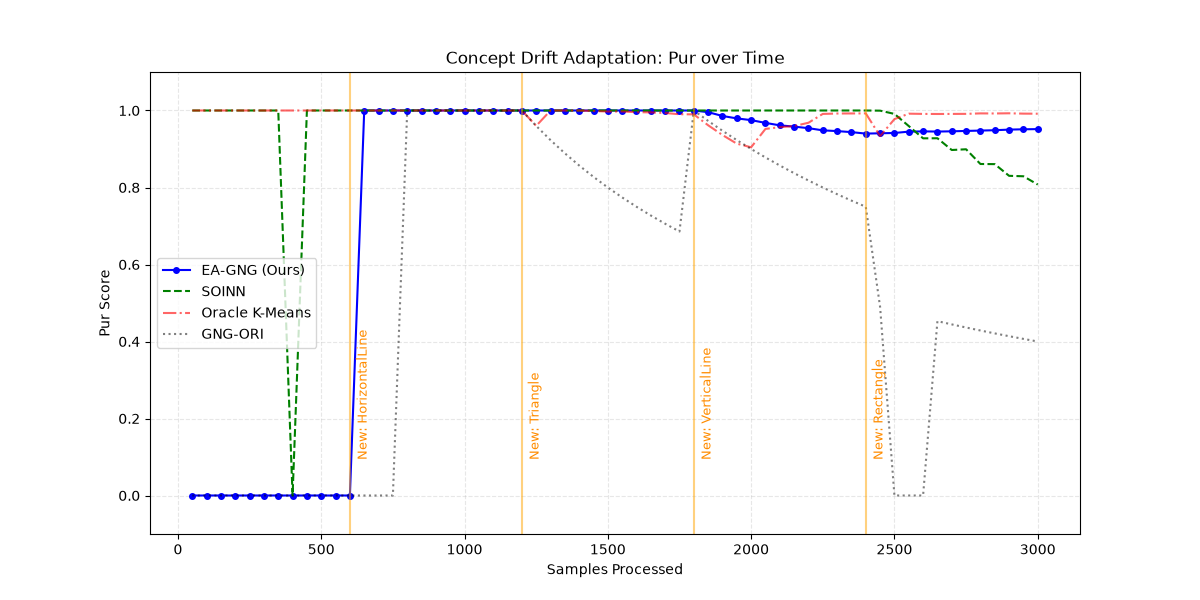
\includegraphics[width=0.9\linewidth]{figures/c4/c4_Pur.png}
    \caption{Chỉ số độ thuần khiết phân cụm của các thuật toán theo từng giai đoạn xuất hiện lỗi.}
    \caption*{Ghi chú: Mức độ thuần khiết phản ánh tỷ lệ mẫu thuộc lớp chiếm ưu thế trong từng cụm tô-pô.}
    \label{fig:drift_pur}
\end{figure}

Độ thuần khiết (Purity) của các cụm được khởi tạo bởi EAGNG thể hiện mức độ chính xác cao trong việc gom nhóm các mẫu lỗi có cùng bản chất kỹ thuật. Như được miêu tả ở Hình~\ref{fig:drift_pur}, độ thuần khiết của EAGNG đạt $95{,}2\%$ tại bước cuối cùng $3000$. Trái lại, phương pháp GNG truyền thống bị giảm độ thuần khiết xuống $40{,}0\%$ do các nơ-ron cũ bị kéo lệch khỏi tâm phân bố gốc khi dữ liệu mới xuất hiện. Sự duy trì độ thuần khiết cao của EAGNG khẳng định hiệu quả của cơ chế điều chỉnh độ linh hoạt dựa trên bằng chứng tích lũy.

\subsection{Phân tích độ ổn định cấu trúc và hiện tượng quên thảm họa}
\label{sec:4_2_2_stability}

Hiện tượng quên thảm họa là thách thức lớn đối với các mô hình học liên tục khi tiếp nhận các phân bố dữ liệu mới. Để đánh giá mức độ suy giảm tri thức cũ, khoảng cách dịch chuyển chuẩn L2 ($\Delta W$) của các nút đã tồn tại được đo đạc và theo dõi qua các bước cập nhật dữ liệu. 

\begin{figure}[htbp]
    \centering
    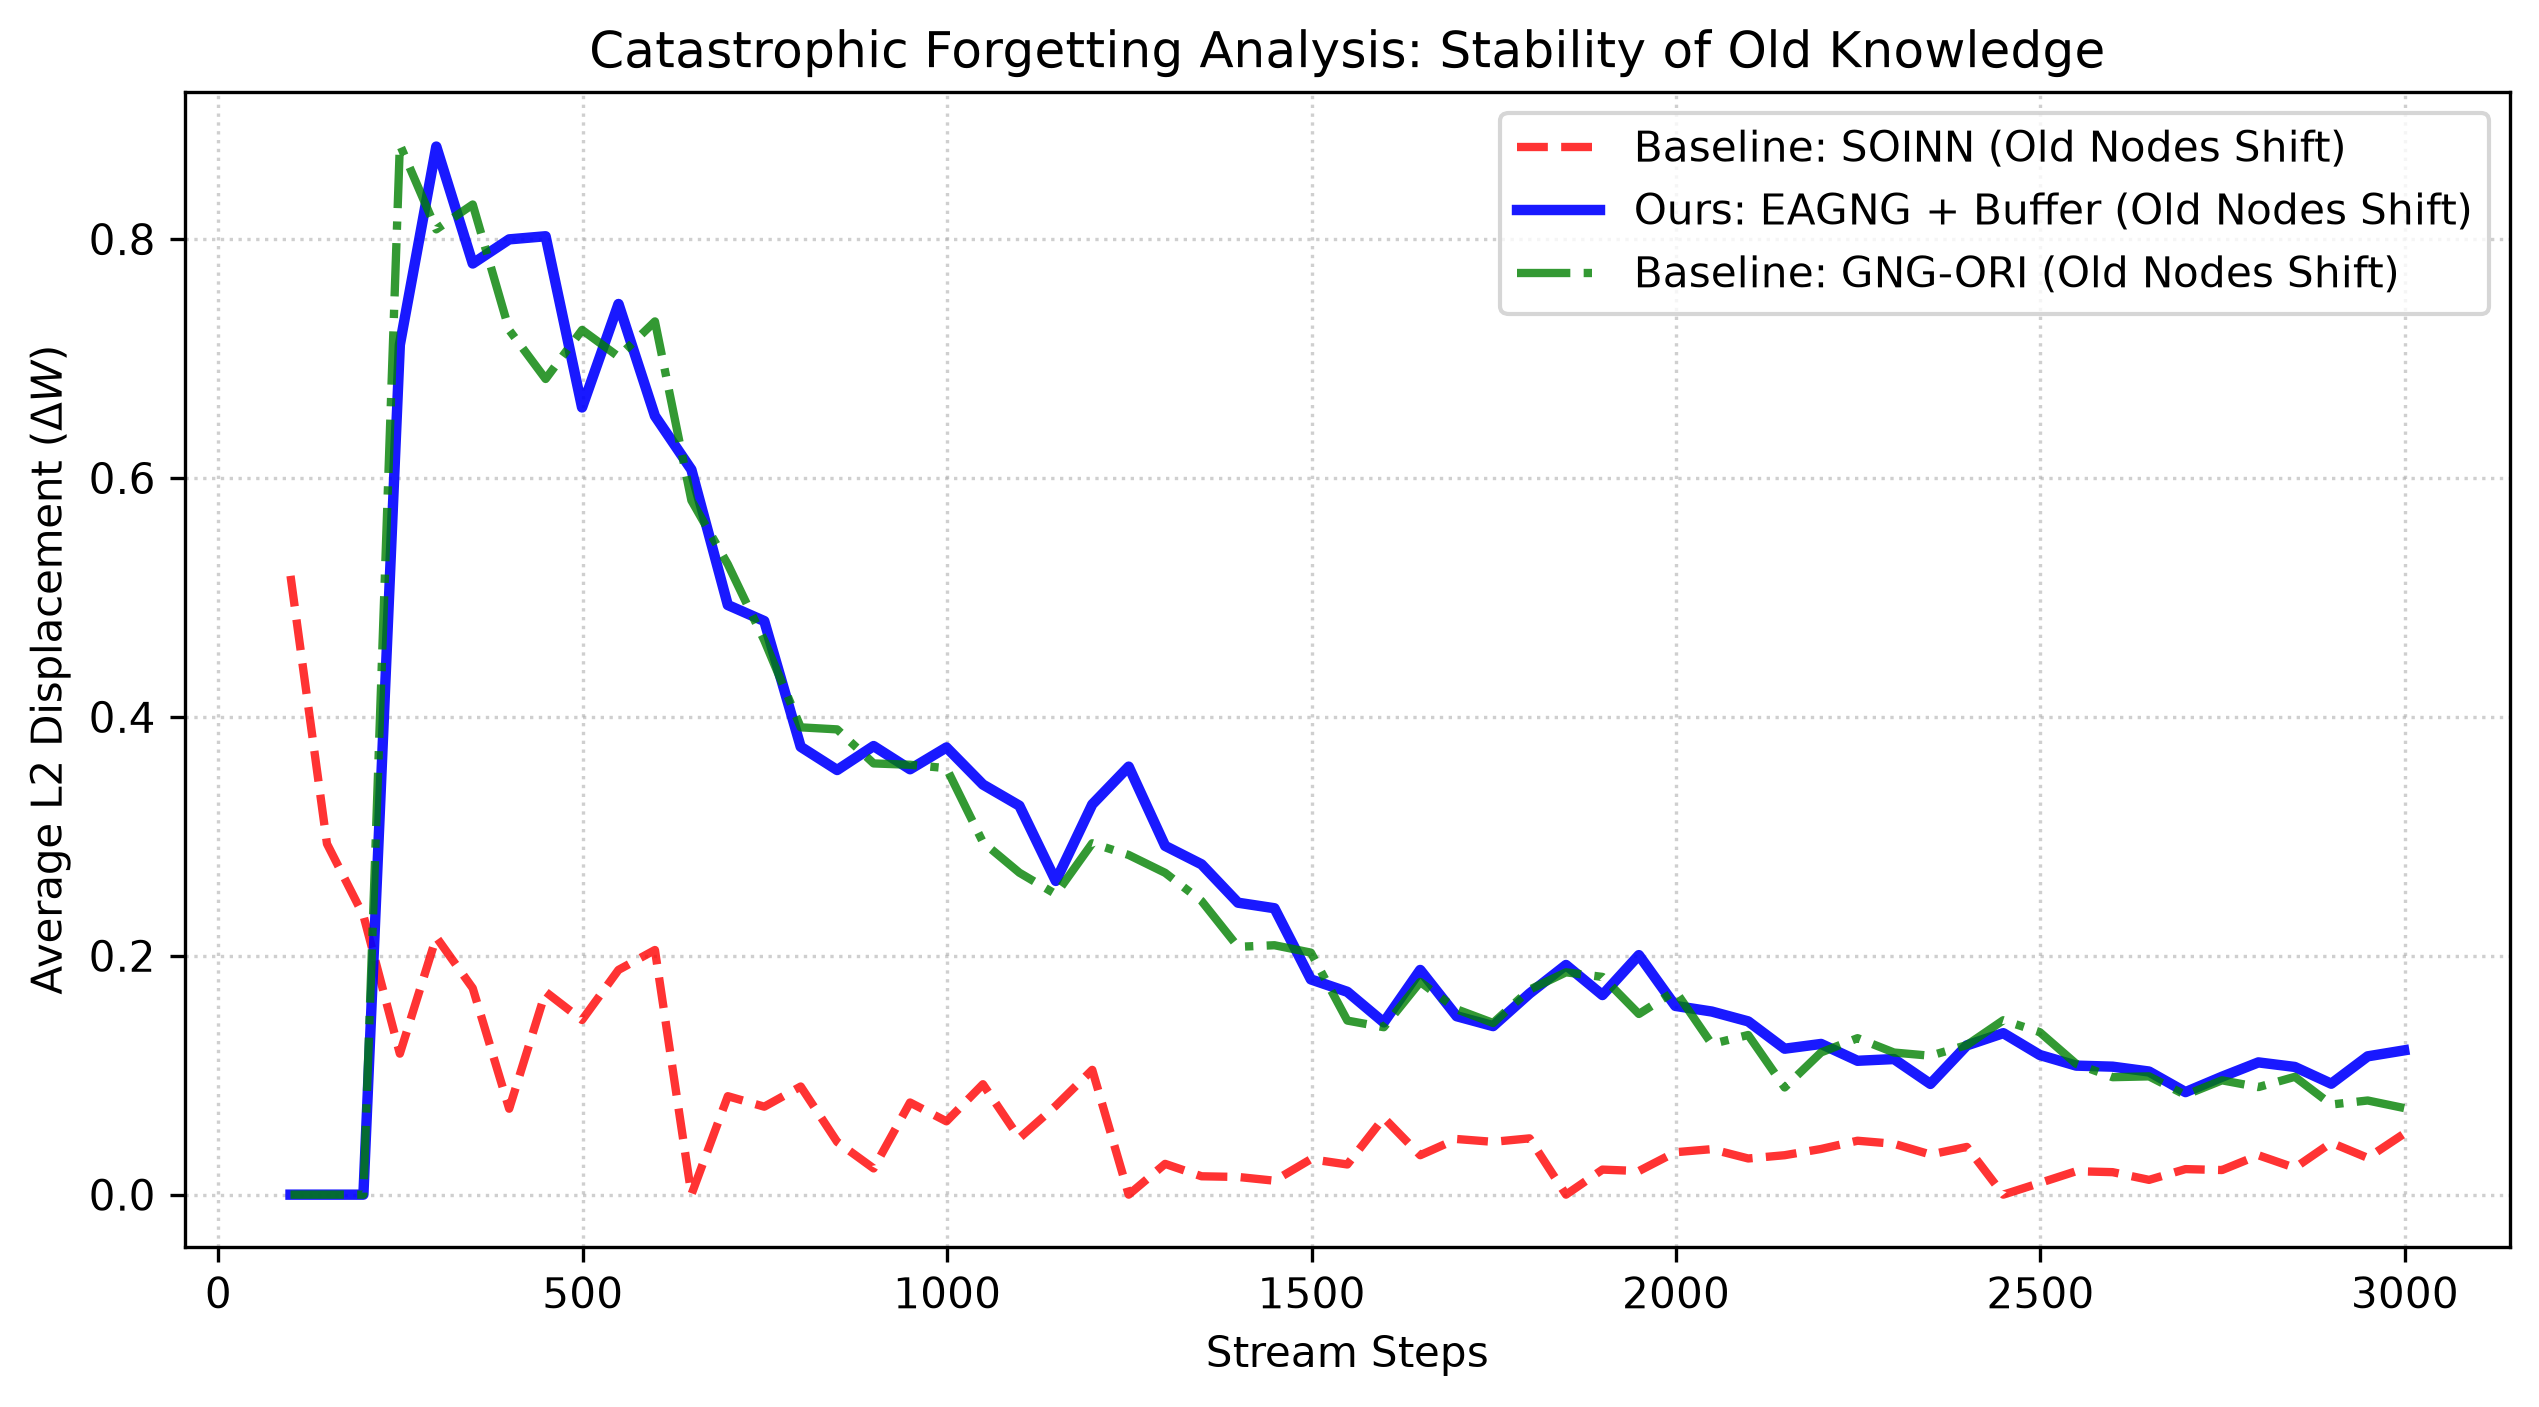
\includegraphics[width=0.85\linewidth]{figures/c4/c4_comparison.png}
    \caption{So sánh độ dịch chuyển trọng số nút cũ giữa các thuật toán theo chuỗi thời gian.}
    \caption*{Ghi chú: Giá trị độ dịch chuyển càng nhỏ thể hiện mức độ bảo toàn tri thức cũ càng cao.}
    \label{fig:stability_comp}
\end{figure}

Hình~\ref{fig:stability_comp} cho thấy mức độ dịch chuyển trọng số nút cũ của EAGNG kết hợp bộ đệm đạt giá trị xấp xỉ $0{,}10$ ở giai đoạn ổn định, thấp hơn đáng kể so với hiện tượng suy biến cấu trúc trong GNG truyền thống. Thuật toán SOINN duy trì mức dịch chuyển nhỏ nhưng đổi lại phải đánh đổi bằng việc khởi tạo quá nhiều nút không cần thiết. Phương pháp EAGNG đạt được sự cân bằng giữa việc tiếp thu tri thức mới và việc bảo toàn tri thức cũ nhờ vào bộ đệm tích lũy bằng chứng.

\begin{figure}[htbp]
    \centering
    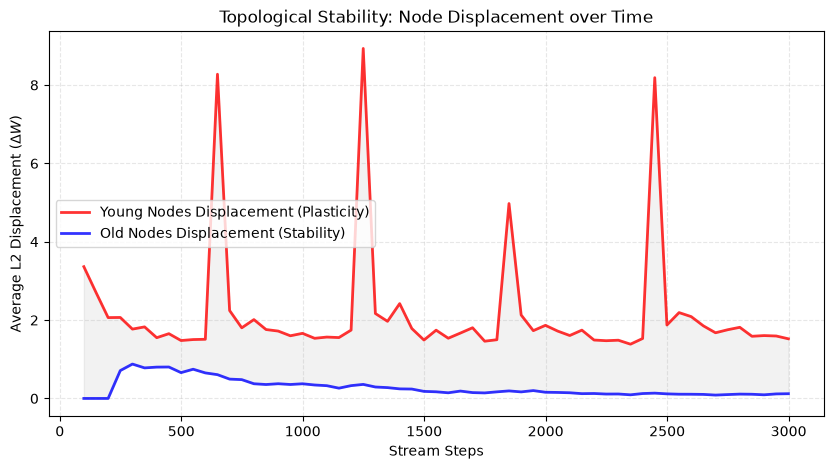
\includegraphics[width=0.85\linewidth]{figures/c4/c4_topological_stability.png}
    \caption{Phân tích khả năng thích ứng linh hoạt và độ ổn định tô-pô của mạng EAGNG.}
    \caption*{Ghi chú: Đường màu đỏ biểu diễn độ dịch chuyển của các nút mới (Plasticity), đường màu xanh biểu diễn độ dịch chuyển của các nút cũ (Stability).}
    \label{fig:topo_stability}
\end{figure}

Sự phân tách rõ rệt giữa tính linh hoạt (Plasticity) và tính ổn định (Stability) được thể hiện rõ ràng trong Công thức và cấu trúc tô-pô của EAGNG. Như miêu tả ở Hình~\ref{fig:topo_stability}, các nút mới (Young Nodes) đạt biên độ dịch chuyển trọng số lên tới $8{,}9$ tại các điểm xảy ra dịch chuyển khái niệm (bước $600$, $1200$, $1800$, $2400$), cho phép mạng thích ứng nhanh chóng với dạng lỗi mới. Trong khi đó, các nút cũ (Old Nodes) duy trì độ dịch chuyển trọng số luôn dưới $0{,}5$, đảm bảo các vùng không gian đại diện cho lỗi đã học không bị biến dạng.

\subsection{Đánh giá thời gian thực thi và tốc độ xử lý}
\label{sec:4_2_3_takt_time}

Tốc độ xử lý của thuật toán phân loại phải đáp ứng yêu cầu thời gian nhịp sản xuất (Takt Time) của dây chuyền kiểm tra màn hình điện thoại thực tế. Các chỉ số về thời gian tích lũy, thời gian xử lý trung bình trên mỗi mẫu (Takt Time), và tốc độ xử lý số mẫu trên giây (Throughput) được đo đạc trực tiếp trên cùng một cấu hình phần cứng.

\begin{figure}[htbp]
    \centering
    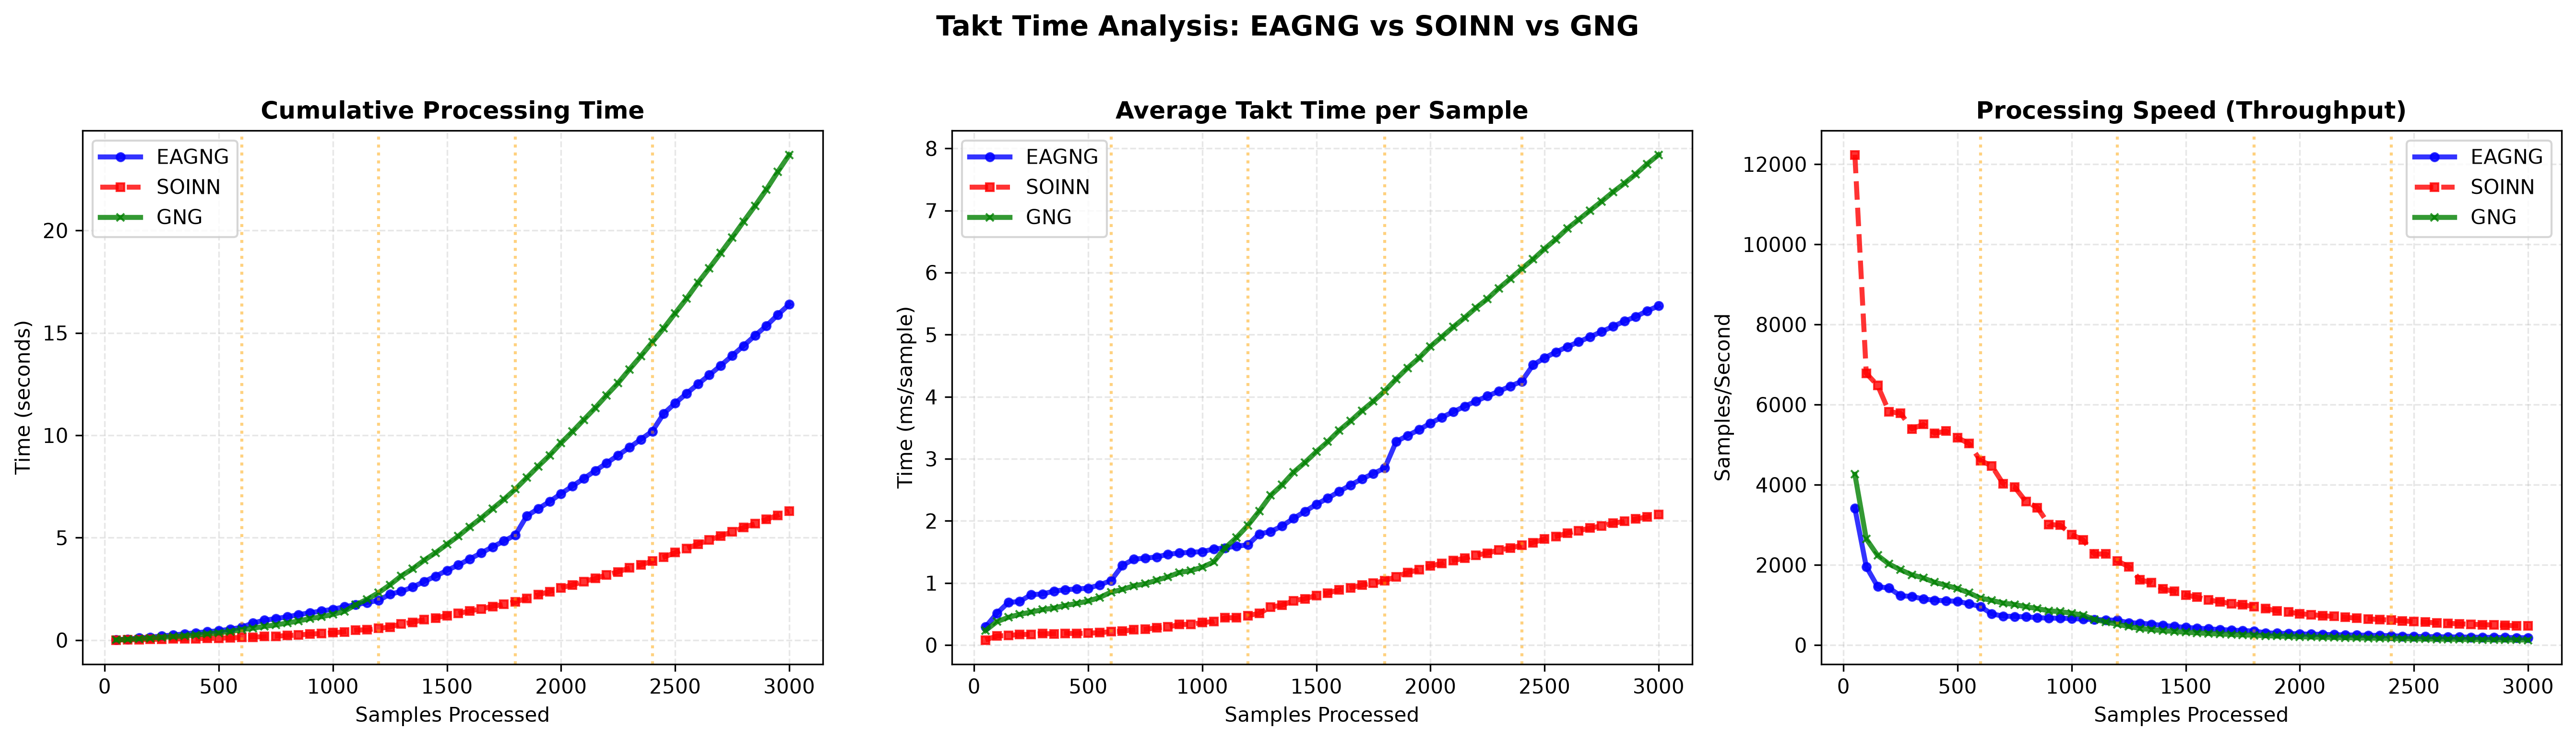
\includegraphics[width=0.98\linewidth]{figures/c4/c4_takt_time.png}
    \caption{Phân tích thời gian nhịp và tốc độ xử lý của EAGNG, SOINN và GNG.}
    \caption*{Ghi chú: Hình bên trái thể hiện thời gian xử lý tích lũy (giây), hình giữa thể hiện thời gian trung bình cho mỗi mẫu (mili-giây), hình bên phải thể hiện tốc độ xử lý (mẫu/giây).}
    \label{fig:takt_time}
\end{figure}

Như thể hiện trong Hình~\ref{fig:takt_time}, thời gian tích lũy của EAGNG đạt $16{,}39$ giây cho $3000$ mẫu, nhanh hơn so với $23{,}69$ giây của GNG truyền thống, dù chậm hơn SOINN ($6{,}30$ giây). Thời gian nhịp xử lý trung bình mỗi mẫu của EAGNG đạt $5{,}46$ mili-giây tại bước $3000$, hoàn toàn đáp ứng ngưỡng thời gian nhịp yêu cầu trong dây chuyền công nghiệp (thường dưới $50$ mili-giây trên mỗi vùng ảnh kiểm tra). Việc kiểm soát số lượng nút ở mức $268$ nút giúp EAGNG duy trì tốc độ xử lý xấp xỉ $183$ mẫu trên giây, tránh hiện tượng bùng nổ chi phí tính toán toán học $O(N^2)$ của các cạnh nối khi mạng phát triển quá lớn.

\subsection{Phân tích trực quan hóa phân cụm lỗi màn hình}
\label{sec:4_2_4_visual_analysis}

Kết quả phân bố không gian biểu diễn hình học của các thuật toán được trực quan hóa nhằm đánh giá khả năng duy trì ranh giới phân cụm đối với dữ liệu lỗi màn hình. Các ảnh trực quan hóa thể hiện cấu trúc đồ thị nút và các cụm lỗi được hình thành tự động tại bước $3000$.

\begin{figure}[htbp]
    \centering
    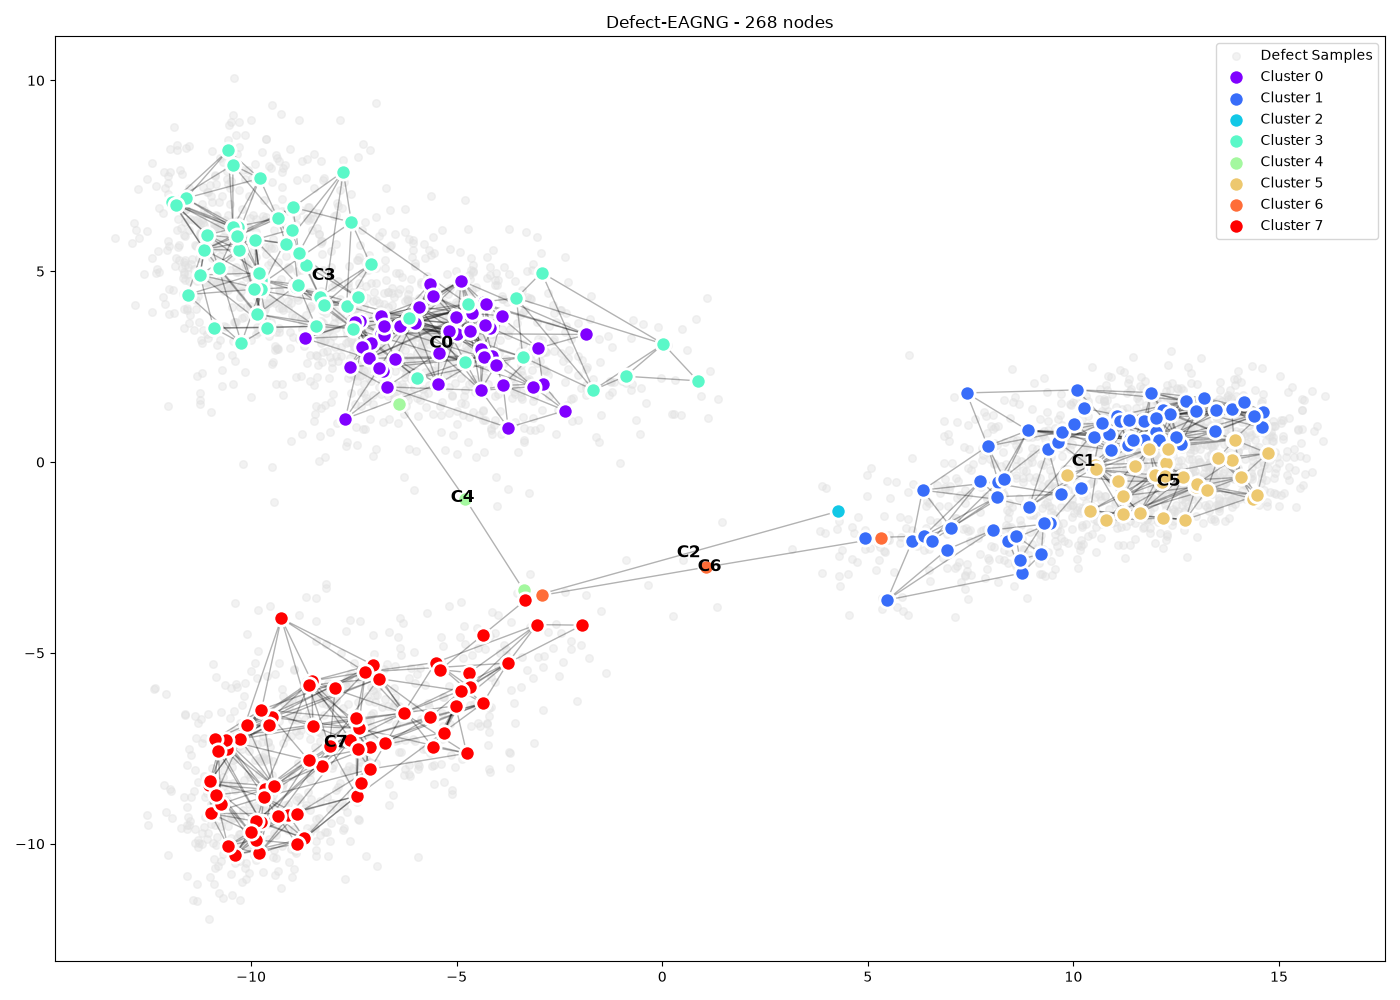
\includegraphics[width=0.85\linewidth]{figures/c4/c4_eagng.png}
    \caption{Trực quan hóa cấu trúc mạng và phân cụm của thuật toán EAGNG tại bước $3000$.}
    \caption*{Ghi chú: Mô hình xây dựng thành công $268$ nút với $8$ cụm phân biệt rõ ràng từ C0 đến C7.}
    \label{fig:vis_eagng}
\end{figure}

Cấu trúc mạng do EAGNG tạo ra thể hiện sự tương thích cao với phân bố tự nhiên của dữ liệu lỗi. Như được thể hiện trong Hình~\ref{fig:vis_eagng}, EAGNG tự động hình thành $268$ nút và tách biệt chính xác $8$ cụm lỗi riêng biệt từ C0 đến C7 mà không cần khai báo trước số lượng cụm. Các cạnh liên kết giữa các nút phản ánh đúng mật độ liên tục của dữ liệu trong từng vùng không gian, trong khi ranh giới giữa các cụm được phân định rõ ràng nhờ cơ chế loại bỏ cạnh lỗi thời.

\begin{figure}[htbp]
    \centering
    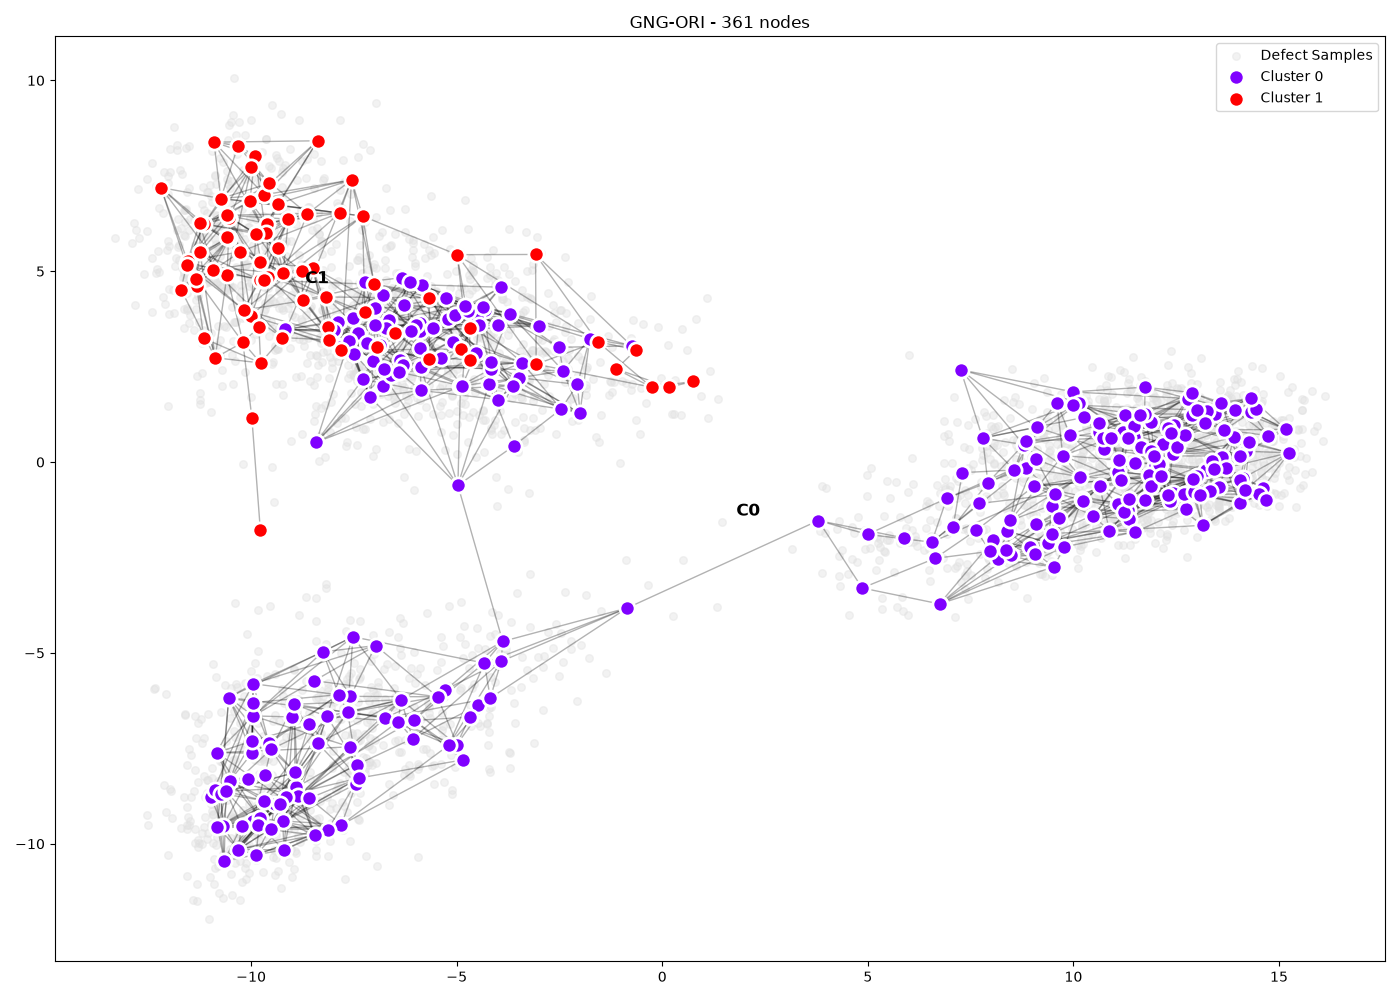
\includegraphics[width=0.85\linewidth]{figures/c4/c4_gng.png}
    \caption{Trực quan hóa cấu trúc mạng của thuật toán GNG truyền thống tại bước $3000$.}
    \caption*{Ghi chú: Mạng phát triển lên $361$ nút nhưng bị gộp thành $2$ cụm lớn không chính xác.}
    \label{fig:vis_gng}
\end{figure}

Ngược lại, cấu trúc của GNG truyền thống bị suy thoái nghiêm trọng dưới tác động của dịch chuyển khái niệm. Như mô tả ở Hình~\ref{fig:vis_gng}, GNG truyền thống khởi tạo tới $361$ nút nhưng chỉ phân tách được $2$ cụm lớn C0 và C1. Các nút mạng nối liền các vùng dữ liệu vốn dĩ thuộc các dạng lỗi khác nhau, dẫn đến hiện tượng trộn lẫn các lớp lỗi và làm giảm chỉ số ARI xuống $21{,}0\%$.

\begin{figure}[htbp]
    \centering
    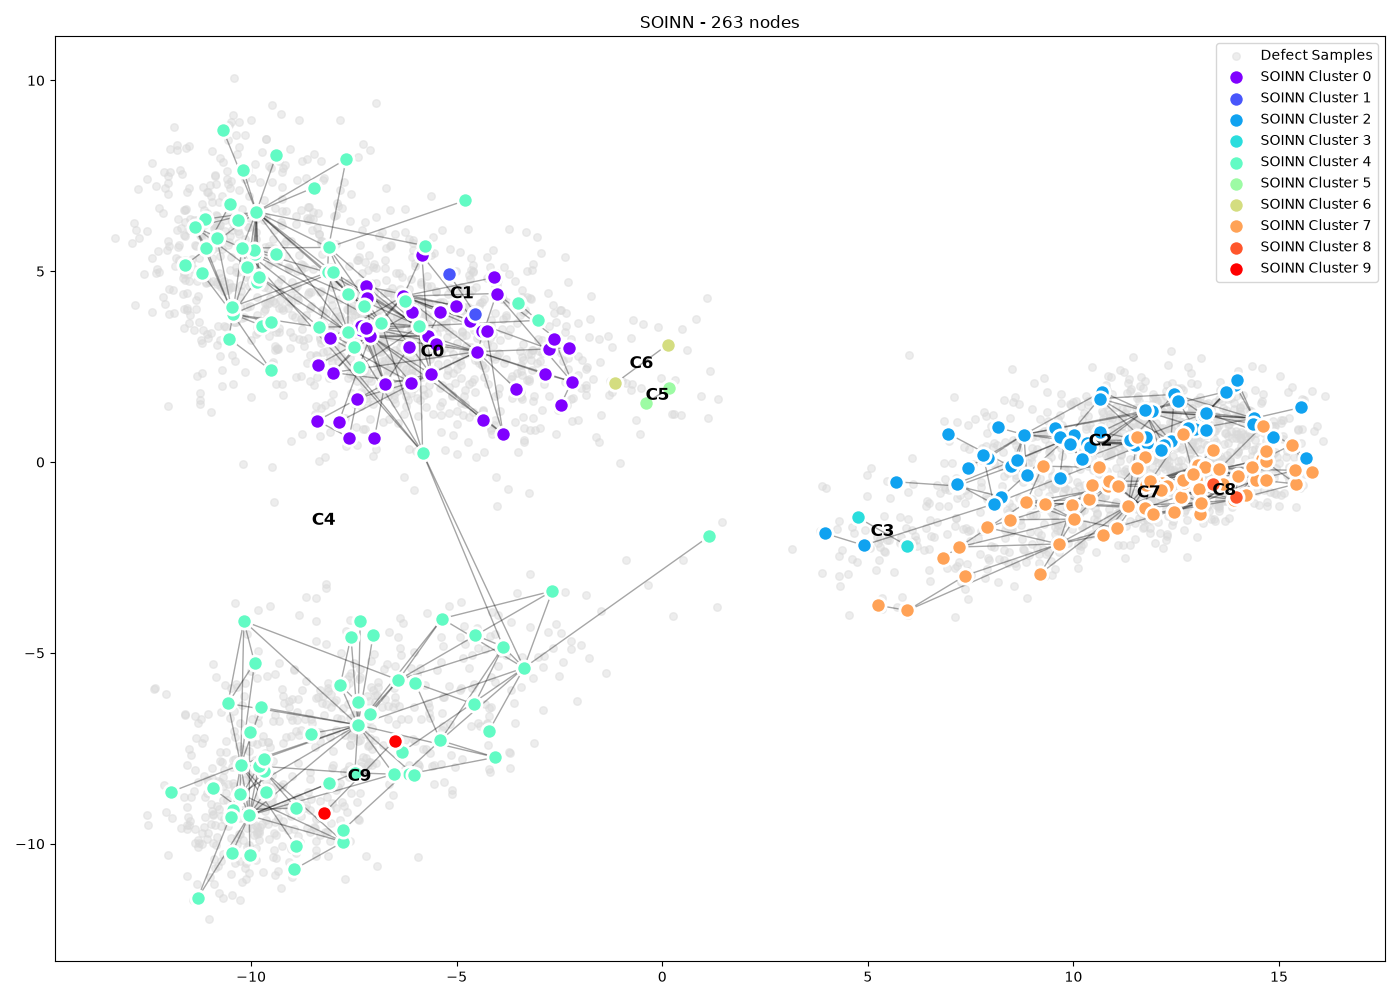
\includegraphics[width=0.85\linewidth]{figures/c4/c4_soinn.png}
    \caption{Trực quan hóa cấu trúc mạng của thuật toán SOINN tại bước $3000$.}
    \caption*{Ghi chú: Mạng khởi tạo $263$ nút nhưng bị phân mảnh thành $10$ cụm do ngưỡng phân tách quá khắt khe.}
    \label{fig:vis_soinn}
\end{figure}

Đối với thuật toán SOINN, mạng gặp phải hiện tượng phân mảnh cụm quá mức. Như thể hiện trong Hình~\ref{fig:vis_soinn}, SOINN tạo ra $263$ nút và chia dữ liệu thành $10$ cụm riêng biệt từ C0 đến C9. Một số cụm nhỏ lẻ bị cô lập hoàn toàn dù thuộc cùng một dạng phân bố lỗi gốc, làm giảm hiệu quả tổng hợp thông tin cho các công đoạn phân loại tự động phía sau.

\subsection{Tổng hợp kết quả so sánh định lượng}
\label{sec:4_2_5_summary}

Bảng~\ref{tab:metrics_summary} tổng hợp các chỉ số đánh giá hiệu năng của phương pháp đề xuất EAGNG so với các phương pháp cơ sở tại thời điểm kết thúc chuỗi thực nghiệm ($3000$ mẫu). Các chỉ số bao gồm chỉ số Rand điều chỉnh (ARI), chỉ số thông tin tương hỗ chuẩn hóa (NMI), độ thuần khiết, số lượng nút mạng, và tổng thời gian tính toán tích lũy. Ngoài ra, kết quả của thuật toán Oracle K-Means \cite{macqueen1967methods} được đưa vào để làm chuẩn mực so sánh, mặc dù phương pháp này yêu cầu gán nhãn trước và không thể áp dụng trực tiếp trong môi trường học trực tuyến. Chính vì vậy, các chỉ số của Oracle K-Means khi biết trước số cụm được xem như giới hạn trên về hiệu năng phân cụm mà các thuật toán học trực tuyến có thể hướng tới.

\begin{table}[htbp]
    \centering
    \caption{Bảng tổng hợp chỉ số hiệu năng định lượng tại thời điểm mẫu thứ $3000$.}
    \label{tab:metrics_summary}
    \begin{tabular}{|l|c|c|c|c|c|}
        \hline
        Phương pháp & ARI & NMI & Độ thuần khiết & Số nút & Thời gian (giây) \\
        \hline
        EAGNG (Đề xuất) & 89,5\% & 92,7\% & 95,2\% & 268 & 16,39 \\
        SOINN \cite{furao2006soinn} & 76,3\% & 87,4\% & 80,8\% & 263 & 6,30 \\
        GNG \cite{fritzke1995growing} & 21,0\% & 47,4\% & 40,0\% & 361 & 23,69 \\
        Oracle K-Means \cite{macqueen1967methods} & 97,9\% & 97,5\% & 99,2\% & - & - \\
        \hline
    \end{tabular}
\end{table}

Các số liệu trong Bảng~\ref{tab:metrics_summary} khẳng định rằng EAGNG đạt sự cân bằng tối ưu giữa chất lượng phân cụm và chi phí tài nguyên tính toán. Thuật toán EAGNG vượt trội hơn SOINN $13{,}2$ điểm phần trăm về chỉ số ARI và $14{,}4$ điểm phần trăm về độ thuần khiết, trong khi tiết kiệm được $30{,}8\%$ thời gian tính toán và giảm $25{,}8\%$ số lượng nút so với GNG truyền thống.